\subsection{Взаимное исключение}

\begin{frame}
	\tableofcontents[currentsection,currentsubsection]
\end{frame}

\begin{frame}{Как избежать гонок}
	\begin{itemize}
		\item Можно обозначить кусок кода как \textit{критическую секцию} (critical section).
		\item Каждую критическую секцию может выполнять максимум один поток.
		\item
			Если весь доступ к общим данным обозначить как критическую секцию,
			то он станет де-факто атомарным.
		\item С каждой критической секцией ассоцириуется \textit{блокировка} (lock).
		\item При входе в секцию блокировку надо \textit{взять}/\textit{захватить} (acquire).
		\item При выходе из секции блокировку надо \textit{отпустить} (unlock/release).
		\item Другие названия блокировок: монитор (monitor), мьютекс (mutex, \textbf{mut}al \text{ex}clusion).
		\item Обычно реализованы на уровне ОС и все операции с ними медленные.
	\end{itemize}
\end{frame}

\begin{frame}[fragile]{Некорректный пример}
\begin{minted}{cpp}
int data;
void* worker(void* arg __attribute__((unused))) {
  pthread_mutex_t m;
  pthread_mutex_init(&m, NULL);
  for (int i = 0; i < N; i++) {
    pthread_mutex_lock(&m);
    data++;
    pthread_mutex_unlock(&m);
  }
  pthread_mutex_destroy(&m);
  return NULL;
}
\end{minted}
\href{https://github.com/yeputons/fall-2016-paradigms/raw/master/161019/sources/09-two-threads-bad-mutex.c}{Код}.
\end{frame}

\begin{frame}[fragile]{Корректный пример}
\begin{minted}{cpp}
int data;
pthread_mutex_t m;
void* worker(void* arg __attribute__((unused))) {
  for (int i = 0; i < N; i++) {
    pthread_mutex_lock(&m);
    data++;
    pthread_mutex_unlock(&m);
  }
  return NULL;
}
// ...
  pthread_mutex_init(&m, NULL);
// ...
  pthread_mutex_destroy(&m);
// ...
\end{minted}
\end{frame}

\begin{frame}{Упражнение}
	\begin{enumerate}
		\item Добавьте mutex в \href{https://github.com/yeputons/fall-2016-paradigms/raw/master/161019/sources/08-two-threads.c}{двойной счётчик}.
		\item Уменьшите $N$ на несколько порядков (mutex'ы сильно замедляют программу).
		\item Убедитесь, что всегда выводится $2N$.
		\item Добавьте mutex в \href{https://github.com/yeputons/fall-2016-paradigms/raw/master/161019/sources/04-writeln-race.c}{writeln}.
	\end{enumerate}
	\href{https://github.com/yeputons/fall-2016-paradigms/raw/master/161019/sources/10-two-threads-good-mutex.c}{Исправленный двойной счётчик},
	\href{https://github.com/yeputons/fall-2016-paradigms/raw/master/161019/sources/11-writeln-mutex.c}{исправленный writeln}.
\end{frame}

\begin{frame}[fragile]{Блокировка}
	\begin{itemize}
		\item \t{pthread\_mutex\_lock} блокируется и ждёт, пока блокировка не станет доступна для захвата.
		\item Есть ли проблемы в следующем псевдокоде?
\begin{minted}{cpp}
void thread1() {
  m1.lock(); m2.lock();
  // ...
  m2.unlock(); m1.unlock();
}
void thread2() {
  m2.lock(); m1.lock();
  // ...
  m1.unlock(); m2.unlock();
}
\end{minted}
	\end{itemize}
\end{frame}

\begin{frame}{Взаимная блокировка}
	\begin{center}
		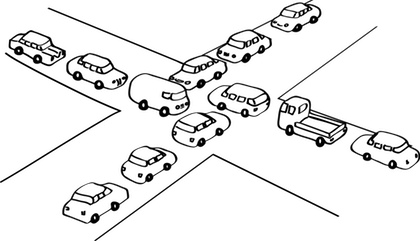
\includegraphics{deadlock.jpg}
	\end{center}
	\begin{itemize}
		\item
			Может случиться проблема:
			\begin{enumerate}
				\item Поток 1 захватывает \t{m1}.
				\item Поток 2 захватывает \t{m2}.
				\item Поток 1 не может захватить \t{m2}.
				\item Поток 2 не может захватить \t{m1}.
				\item Оба потока встали в \textit{deadlock} (\textit{взаимная блокировка}).
			\end{enumerate}
		\item
			Решение: всегда брать блокировки в одном и том же порядке.
			Тогда можно доказать, что deadlock такого вида не образуется.
		\item
			Если ввести линейный порядок на mutex не получается, у вас проблема.
	\end{itemize}
\end{frame}

\begin{frame}[fragile]{Reentrant}
\begin{minted}{cpp}
void inc() {
  m.lock(); data++; m.unlock();
}
void double_inc() {
  m.lock(); inc(); inc(); m.unlock();
}
\end{minted}
	\begin{itemize}
		\item \t{double\_inc} заблокируется, так как \t{inc} попробует взять mutex второй раз.
		\item Есть специальный вид mutex, которые позволяют захватывать себя ещё раз из того же потока, называется \textit{reentrant}.
		\item Их обычно не используют "--- они сложнее в реализации.
		\item
			Решение: ввести <<приватную>> функцию \t{inc\_lock\_held}, которая предполагает,
			что mutex уже взят.
	\end{itemize}
\end{frame}

\begin{frame}{Резюме}
	\begin{itemize}
		\item Атомарные операции в потоках могут выполняться в любом порядке, если их не синхронизировать.
		\item Вы обычно не знаете, что атомарно, а что нет.
		\item \textit{Любой} доступ к общим ресурсам должен быть \textit{защищён} (guarded) блокировкой.
		\item Блокировки надо брать всегда в одном и том же порядке.
		\item TODO
	\end{itemize}
\end{frame}

\begin{frame}{Иллюстрация}
	
\end{frame}
